\section*{BÀI TẬP CUỐI CHƯƠNG 2}

\subsection{Câu hỏi trắc nghiệm}

\Opensolutionfile{ans}[ans/ans-8C2-OTC]

%Câu 1
\begin{ex}%[Dự án EX-8-Đề Cương Toán 8]%[Huu Son]%[8H1N1-1]
	Hình nào sau đây là hình chóp tam giác đều?
	\choice
	{Hình có đáy là tam giác}
	{Hình có đáy là tam giác đều}
	{\True Hình có đáy là tam giác đều và tất cả các cạnh bên bằng nhau}
	{Hình có đáy là tam giác đều và 1 cạnh bên bằng cạnh đáy}
	\loigiai{
		Hình có đáy là tam giác đều và tất cả các cạnh bên bằng nhau là hình chóp đều.
	}
\end{ex}

%Câu 2
\begin{ex}%[Dự án EX-8-Đề Cương Toán 8]%[Huu Son]%[8H1N1-1]
	Hình chóp tam giác đều có mặt bên là
	\choice
	{Tam giác vuông}
	{Tam giác vuông cân}
	{Tam giác đều}
	{\True Tam giác cân}
	\loigiai{
	Hình chóp tam giác đều có mặt bên là tam giác cân.
	}
\end{ex}

%Câu 3
\begin{ex}%[Dự án EX-8-Đề Cương Toán 8]%[Huu Son]%[8H1N1-1]
	Hình chóp tam giác đều có đáy là
	\choice
	{Hình vuông}
	{Hình bình hành}
	{\True Tam giác đều}
	{Hình thang cân}
	\loigiai{
	Hình chóp tam giác đều có đáy là hình tam giác đều.
	}
\end{ex}

%Câu 4
\begin{ex}%[Dự án EX-8-Đề Cương Toán 8]%[Huu Son]%[8H1N1-1]
\immini[thm]{
	Số mặt bên của hình chóp tam giác đều là
	\choice
	{$4$}
	{\True $3$}
	{$2$}
	{$1$}
}
{
\begin{tikzpicture}[line join=round, line cap=round, font=\small, scale=0.6]
\path
	(0:0) coordinate (A)
	($(A)+(-68:2.1)$) coordinate (B)
	($(A)+(0:4)$) coordinate (C)
	($(A)!.5!(B)$) coordinate (O1)
	($(A)!.5!(C)$) coordinate (O2)
	(intersection of C--O1 and B--O2) coordinate (O)
	(O)++(90:4.2) coordinate (S)
;
\draw[dashed] (A)--(C);
\draw 
	(A)--(B)--(C)
	(A)--(S)--(B) (S)--(C)
;
\foreach \x/\g/\t in {A/180/A,B/-90/B,C/0/C,S/90/S} 
	\draw[fill=black] (\x) circle (.05) +(\g:.3) node{$\x$};		%0.05
\end{tikzpicture}
}
	\loigiai{
	Hình chóp tam giác đều có $3$ mặt bên và $1$ mặt đáy.
	}
\end{ex}

%Câu 5
\begin{ex}%[Dự án EX-8-Đề Cương Toán 8]%[Huu Son]%[8H1N1-1]
\immini[thm]{
	Chiều cao của tam giác mặt bên kẻ từ đỉnh của hình chóp tam giác đều trong hình bên là
	\choice
	{$SB$}
	{$SH$}
	{\True $SI$}
	{$BI$}
}
{
\begin{tikzpicture}[scale=0.6,>=stealth, font=\footnotesize, line join=round, line cap=round]
	\path 
		(0,0) coordinate (B) 
		(4,-2) coordinate (A)
		(6,0) coordinate (C)
		(3,4) coordinate (S)
		(5,-1) coordinate (I)
		(3,-0.6) coordinate (H)
	;
	\draw (S)--(B)--(A)--(C)--(S) --(A); 
	\draw (S)--(I);
	\draw [dashed] (I)--(B)--(C);
	\draw [dashed] (S)--(H);
	\foreach \p/\r in {S/90,B/180,A/-90,C/0, I/0, H/-90}
	\fill (\p) circle (.05) node[shift={(\r:3mm)}]{$\p$};
	\foreach \x/\y/\z in {S/I/C,S/H/B}
		\draw pic[draw,angle radius=2mm]{right angle=\x--\y--\z};
\end{tikzpicture}
}
	\loigiai{		
		Ta có trung đoạn của hình chóp là $SI$.}
\end{ex}

%Câu 6
\begin{ex}%[Dự án EX-8-Đề Cương Toán 8]%[Huu Son]%[8H1N1-1]
	Hình nào trong các hình sau là hình chóp tứ giác đều?
\begin{center}
	\begin{tabular}{cccc}
		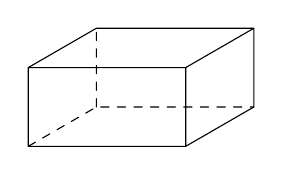
\begin{tikzpicture}[line join=round, line cap=round, font=\small, scale=1]
		\path
			(0,0) coordinate (A)
			(2,0) coordinate (B)
			(A)+(30:1) coordinate (D)
			(B)+(30:1) coordinate (C);
		\foreach \d in {A, B, C, D}
			\path (\d)+(90:1) coordinate (\d1);
		\draw 
			(A1)--(B1)--(C1)--(D1)--cycle 
			(A)--(A1) (B)--(B1) (C)--(C1) (A)--(B)--(C);
		\draw[dashed] (A)--(D)--(C) (D)--(D1);
		\end{tikzpicture}
		&
		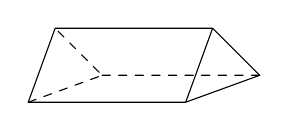
\begin{tikzpicture}[line join=round, line cap=round, font=\small, scale=1]
		\path 
			(0,0) coordinate (A)
			(20:1) coordinate (B)
			(70:1) coordinate (C)
		;
		\foreach \d in {A,B,C}{
			\path (\d)+(180:2) coordinate (\d1);
		}
		\draw (A)--(B)--(C)--cycle (A)--(A1)--(C1)--(C)--cycle;
		\draw[dashed] (B)--(B1) (A1)--(B1)--(C1);
		\end{tikzpicture}
		&
		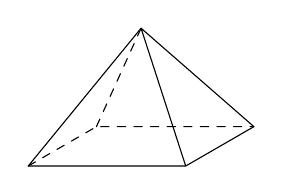
\begin{tikzpicture}[line join=round, line cap=round, font=\small, scale=1]
		\path 
			(0,0) coordinate (A)
			(2,0) coordinate (B)
			(B)+(30:1) coordinate (C)
			(A)+(30:1) coordinate (D) 
			(intersection of A--C and B--D) coordinate (O)
			+(90:1.5) coordinate (S)
		;
		\draw (S)--(A)--(B)--(C)--cycle (S)--(B);
		\draw[dashed] (A)--(D)--(C) (D)--(S);
		\end{tikzpicture}
		&
		\begin{tikzpicture}[line join=round, line cap=round, font=\small, scale=1]
		\path
			(0,0) coordinate (A)
			(20:1) coordinate (B)
			(160:1) coordinate (C)
			($(B)!1/2!(C)$) coordinate (M)
			($(A)!2/3!(M)$) coordinate (O)+(90:1.5) coordinate (S)
		;
		\draw (S)--(C)--(A)--(B)--cycle (S)--(A);
		\draw[dashed] (B)--(C);
		\end{tikzpicture}
		\\
		{\small Hình $1$} & {\small Hình $2$} & {\small Hình $3$} & {\small Hình $4$} 
	\end{tabular}
\end{center}
	\choice
	{Hình $1$}
	{Hình $2$}
	{\True Hình $3$}
	{Hình $4$}
	\loigiai{
		Hình $3$ là hình chóp tứ giác đều.
	}
\end{ex}

%Câu 7
\begin{ex}%[Dự án EX-8-Đề Cương Toán 8]%[Huu Son]%[8H1N1-1]
	Hình chóp tứ giác đều có mặt bên là hình gì?
	\choice
	{\True Tam giác cân}
	{Tam giác đều}
	{Tam giác vuông}
	{Hình vuông}
	\loigiai{
		Hình chóp tứ giác đều có mặt bên là hình tam giác cân.
	}
\end{ex}

%Câu 8
\begin{ex}%[Dự án EX-8-Đề Cương Toán 8]%[Huu Son]%[8H1N1-1]
	Hình chóp tứ giác đều có mặt đáy là
	\choice
	{Tam giác cân}
	{\True Hình vuông}
	{Tam giác vuông}
	{Tam giác đều}
	\loigiai{
		Hình chóp tứ giác đều có mặt đáy là hình vuông.
	}
\end{ex}

%Câu 9
\begin{ex}%[Dự án EX-8-Đề Cương Toán 8]%[Huu Son]%[8H1N1-1]
\immini[thm]{
	Cho hình chóp tứ giác đều $S.ABCD$ ở hình bên, khi đó $SH$ được gọi là
	\choice
	{\True Đường cao}
	{Cạnh đáy}
	{Cạnh bên}
	{Đường chéo}
}
{
\begin{tikzpicture}[line join=round, line cap=round, font=\footnotesize, scale=0.6]
\path
	(0:0) coordinate (A)
	++(0:4) coordinate (B)
	++(34:3) coordinate (C)
	($(A)+(C)-(B)$) coordinate (D)
	($(A)!.5!(C)$) coordinate (H)
	(H)++(90:4.5) coordinate (S)
;
\draw[dashed]
	(A)--(D)--(C)--cycle
	(B)--(D)--(S)--(H)
;
\draw
	(A)--(B)--(C)
	(A)--(S)--(B) (S)--(C)
;
\draw pic[draw,angle radius=2mm]{right angle=S--H--C};
\foreach \x/\g/\t in {A/-135/A,B/-45/B,C/0/C,D/150/D,S/90/S,H/-90/H} 
	\draw[fill=black] (\x) circle (.05) +(\g:.4) node{$\x$};		%0.05
\end{tikzpicture}
}
	\loigiai{
		Trong hình chóp tứ giác đều $S.ABCD$ ở hình bên, $SH$ được gọi là đường cao.
	}
\end{ex}

%Câu 10
\begin{ex}%[Dự án EX-8-Đề Cương Toán 8]%[Huu Son]%[8H1H1-1]
Cho hình chóp tam giác đều $S.ABC$, $SH$ là đường cao. Phát biểu nào sau đây là \textbf{sai}?
	\choice
	{$AB=BC=CA$}
	{$SA=SB=SC$}
	{\True $\triangle SAB$, $\triangle SAC$, $\triangle SBC$ là các tam giác đều}
	{$H$ là trọng tâm mặt đáy}
	\loigiai{
	$\triangle SAB$, $\triangle SAC$, $\triangle SBC$ là các tam giác cân tại $S$.
	}
\end{ex}

%Câu 11
\begin{ex}%[Dự án EX-8-Đề Cương Toán 8]%[Huu Son]%[8H4H1-5]
\immini[thm]{
	Cho hình chóp tam giác đều $S.ABC$ có $SH$ là chiều cao. Phát biểu nào sau đây là \textbf{sai}?
	\choice
	{$SA=SB=SC$}
	{$\triangle ABC$ là tam giác đều}
	{\True Diện tích toàn phần của hình chóp bằng ba lần diện tích tam giác $SAB$}
	{Điểm $H$ là trọng tâm của tam giác $ABC$}
}
{
\begin{tikzpicture}[font=\footnotesize,line join=round, line cap=round, >=stealth]
	\path
		(0,0) coordinate (A)
		(3.5,0) coordinate (C)
		(-60:2) coordinate (B)
		($(A)!0.5!(C)$) coordinate (B1)
		($(A)!0.5!(B)$) coordinate (C1)
		($(B)!0.5!(C)$) coordinate (A1)
		(intersection of A--A1 and C--C1) coordinate (H)
		($(H)+(90:3)$) coordinate (S)
	;
	\draw (A)--(B)--(C) (A)--(S)--(B) (S)--(C);
	\draw[dashed] (S)--(H) (C)--(A)--(A1) (B)--(B1);
	\foreach\i/\j in {A/135,C/0,B/-135,S/90,H/-80} 
		\draw[fill=black] (\i) circle (1pt) node[shift=(\j:2.5mm)] {$\i$};	% 1pt
	\draw pic[draw, angle radius=2mm]{right angle=S--H--A};
\end{tikzpicture}
}
	\loigiai{
	Diện tích toàn phần của hình chóp bằng tổng diện tích xung quanh và diện tích đáy nên phát biểu “Diện tích toàn phần của hình chóp bằng ba lần diện tích tam giác $SAB$” là sai.
}
\end{ex}

%Câu 12
\begin{ex}%[Dự án EX-8-Đề Cương Toán 8]%[Huu Son]%[8H1N1-1]
\immini[thm]{
	Hình chóp tứ giác đều $S.ABCD$ có
	\choice
	{$AB$ là đường cao}
	{$SO$ là cạnh đáy}
	{$\triangle SBD$ là mặt bên}
	{\True $SA$ là cạnh bên}
}
{
\begin{tikzpicture}[line join=round, line cap=round, font=\footnotesize, scale=0.6]
\path
	(0:0) coordinate (A)
	++(0:4) coordinate (B)
	++(34:3) coordinate (C)
	($(A)+(C)-(B)$) coordinate (D)
	($(A)!.5!(C)$) coordinate (H)
	(H)++(90:4.5) coordinate (S)
;
\draw[dashed]
	(A)--(D)--(C)--cycle
	(B)--(D)--(S)--(H)
;
\draw
	(A)--(B)--(C)
	(A)--(S)--(B) (S)--(C)
;
\draw pic[draw,angle radius=2mm]{right angle=S--H--C};
\foreach \x/\g/\t in {A/-135/B,B/-45/C,C/0/D,D/150/A,S/90/S,H/-90/O} 
	\draw[fill=black] (\x) circle (.05) +(\g:.4) node{$\t$};		%0.05
\end{tikzpicture}
}
	\loigiai{
		Hình chóp tứ giác đều $S.ABCD$ có $SA$ là cạnh bên.
	}
\end{ex}

%Câu 13
\begin{ex}%[Dự án EX-8-Đề Cương Toán 8]%[Huu Son]%[8H1H2-1]
	Hình chóp tam giác đều có cạnh đáy là $4$ cm và chiều cao của mặt bên tương ứng với cạnh đáy là $3$ cm có diện tích xung quanh là  
	\choice
	{$6$ cm$^2$}
	{\True $18$ cm$^2$}
	{$24$ cm$^2$}
	{$36$ cm$^2$}
	\loigiai{ 
	Diện tích xung quanh của hình chóp tứ giác đều là
	$$\dfrac{1}{2}\cdot(3 \cdot 4)\cdot3=18\,\left(\text{cm}^2\right).$$
	}
\end{ex} 

%Câu 14
\begin{ex}%[Dự án EX-8-Đề Cương Toán 8]%[Huu Son]%[8H1H2-2]
\immini[thm]{
	Cho hình chóp tứ giác đều $S.ABCD$, điểm $O$ là giao điểm hai đường chéo của mặt đáy. Khi đó, thể tích của hình chóp này là
	\choice
	{\True $V=\dfrac{1}{3}SO \cdot S_{ABCD}$}
	{$V=\dfrac{1}{3}SA \cdot S_{ABCD}$}
	{$V=\dfrac{1}{2}SO \cdot S_{ABCD}$}
	{$V=\dfrac{1}{2}SA \cdot S_{ABCD}$}
}
{
\begin{tikzpicture}[line join=round, line cap=round, font=\footnotesize, scale=0.6]
\path
	(0:0) coordinate (A)
	++(0:4) coordinate (B)
	++(34:3) coordinate (C)
	($(A)+(C)-(B)$) coordinate (D)
	($(A)!.5!(C)$) coordinate (H)
	(H)++(90:4.5) coordinate (S)
;
\draw[dashed]
	(A)--(D)--(C)--cycle
	(B)--(D)--(S)--(H)
;
\draw
	(A)--(B)--(C)
	(A)--(S)--(B) (S)--(C)
;
\draw pic[draw,angle radius=2mm]{right angle=S--H--C};
\foreach \x/\g/\t in {A/-135/B,B/-45/C,C/0/D,D/150/A,S/90/S,H/-90/O} 
	\draw[fill=black] (\x) circle (.05) +(\g:.4) node{$\t$};		%0.05
\end{tikzpicture}
}
	\loigiai{
	Thể tích hình chóp tứ giác đều $S.ABCD$ là $V=\dfrac{1}{3}h\cdot S_\text{đáy}=\dfrac{1}{3}SO\cdot S_{ABCD}$.
}
\end{ex}

%Câu 15
\begin{ex}%[Dự án EX-8-Đề Cương Toán 8]%[Huu Son]%[8H1H2-2]
\immini[thm]{
	Cho hình chóp tứ giác đều $I.ABCD$ có độ dài cạnh đáy là $14$ cm và chiều cao là $18$ cm. Thể tích của hình chóp tứ giác đều này là
	\choice
	{$196$ cm$^3$}
	{\True $1\,176$ cm$^3$}
	{$168$ cm$^3$}
	{$3\,528$ cm$^3$}
}
{
\begin{tikzpicture}[line join=round, line cap=round, font=\footnotesize, scale=0.75]
\path
	(0:0) coordinate (A)
	++(0:4) coordinate (B)
	++(34:3) coordinate (C)
	($(A)+(C)-(B)$) coordinate (D)
	($(A)!.5!(C)$) coordinate (H)
	(H)++(90:4.5) coordinate (S)
;
\draw[dashed]
	(A)--(D)--(C)--cycle
	(B)--(D)--(S) (H)--(S)node[midway,rotate=90,above]{\scriptsize $18$ cm}
;
\draw
	(A)--(B)node[midway,below]{\scriptsize $14$ cm}--(C)
	(A)--(S)--(B) (S)--(C)
;
\draw pic[draw,angle radius=2mm]{right angle=S--H--C};
\foreach \x/\g/\t in {A/-135/A,B/-45/B,C/0/C,D/150/D,S/90/I,H/-100/H} 
	\draw[fill=black] (\x) circle (.05) +(\g:.4) node{$\t$};		%0.05
\end{tikzpicture}
}
	\loigiai{
Diện tích đáy hình vuông là $S_{ABCD}=14^2=196$ (cm$^2$). \\
Thể tích hình chóp tứ giác đều $I.ABCD$ là $V=\dfrac{1}{3} \cdot 18 \cdot 196 =1\,176$ (cm$^3$).
	}
\end{ex}

%Câu 16
\begin{ex}%[Dự án EX-8-Đề Cương Toán 8]%[Huu Son]%[8H1H1-1]
	Cho hình chóp tứ giác đều có chiều cao là $7$ cm, độ dài cạnh đáy là $12$ cm. Thể tích của hình chóp tứ giác đều này là
	\choice
	{$336$ cm$^2$}
	{$504$ cm$^2$}
	{\True $336$ cm$^3$}
	{$504$ cm$^3$}
	\loigiai{
	Thể tích của hình chóp tứ giác đều này là $V = \dfrac{1}{3} \cdot 12^2 \cdot 7 = 336$ (cm$^3$).
	}
\end{ex}

%Câu 17
\begin{ex}%[Dự án EX-8-Đề Cương Toán 8]%[Huu Son]%[8H1V2-3]
\immini[thm]{
	Kim tự tháp Kheops ở Ai Cập có dạng hình chóp đều, đáy là hình vuông, các mặt bên là các tam giác cân chung đỉnh (hình vẽ bên). Biết chiều cao của kim tự tháp khoảng $140$ mét, cạnh đáy của nó dài $240$ mét. Tính thể tích của kim tự tháp này.
}
{
\begin{tabular}{cc}
	\begin{tikzpicture}[line join = round, line cap=round,>=stealth,font=\footnotesize,scale=.8]
		\fill[orange!40!white](0,0)--(3,-0.5)--(3.5,4)--cycle;
		\fill[pattern=bricks, pattern color=gray](0,0)--(3,-0.5)--(3.5,4)--cycle;
		\fill[orange!80!black] (3,-0.5)--(3.5,4)--(7,0)--cycle;
		\fill[pattern=bricks] (3,-0.5)--(3.5,4)--(7,0)--cycle;
		\draw 
			(0,0)--(3,-0.5)--(7,0) --(3.5,4)--cycle
			(3,-0.5)--(3.5,4)
		;
	\end{tikzpicture}
&  
\begin{tikzpicture}[line join=round, line cap=round, font=\footnotesize, scale=0.6]
\path
	(0:0) coordinate (A)
	++(0:4) coordinate (B)
	++(34:3) coordinate (C)
	($(A)+(C)-(B)$) coordinate (D)
	($(A)!.5!(C)$) coordinate (H)
	(H)++(90:4.5) coordinate (S)
;
\draw[dashed]
	(A)--(D)--(C)--cycle
	(B)--(D)--(S)--(H)
;
\draw
	(A)--(B)node[midway,below]{\scriptsize $14$ cm}--(C)
	(A)--(S)--(B) (S)--(C)
;
\draw pic[draw,angle radius=2mm]{right angle=S--H--C};
\foreach \x/\g/\t in {A/-135/A,B/-45/B,C/0/C,D/150/D,S/90/S,H/-100/O} 
	\draw[fill=black] (\x) circle (.05) +(\g:.4) node{$\t$};		%0.05
\end{tikzpicture}
\end{tabular}
}
	\choice
	{$2\,687\,000$ m$^3$}
	{\True $2\,688\,000$ m$^3$}
	{$2\,689\,000$ m$^3$}
	{$8\,064\,000$ m$^3$}
	\loigiai{
		Thể tích của kim tự tháp này là $V=\dfrac{1}{3}\cdot 240^2 \cdot 140=2\,688\,000$ (m$^3$).
	}
\end{ex}

\subsection{Bài tập tự luận}

% Bài 1
\begin{bt}%[Dự án EX-8-Đề Cương Toán 8]%[Huu Son]%[8H1H2-1]
\immini[thm]{
	Cho hình chóp tam giác đều $S.ABC$ có độ dài cạnh đáy $AB$ bằng $7$ cm và đường cao của tam giác cân $SAB$ là $SM=11$ cm. Tính diện tích xung quanh của hình chóp tam giác đều này.
}
{
\begin{tikzpicture}[line join=round, line cap=round, font=\footnotesize, scale=0.75]
\path
	(0:0) coordinate (A)
	($(A)+(-28:3.1)$) coordinate (B)
	($(A)+(0:4)$) coordinate (C)
	($(A)!.5!(B)$) coordinate (O1)
	($(B)!.5!(C)$) coordinate (O2)
	(intersection of C--O1 and A--O2) coordinate (O)
	(O)++(90:4.2) coordinate (S)
	(A)--(B)--([turn]-90:0.5cm) coordinate (B1)
	(B)--(A)--([turn]90:0.5cm) coordinate (A1)
	(A1)--(B1)node[midway,sloped,below]{$7$ cm}
	(O1)--(S)node[midway,sloped,above]{$11$ cm}
;
\draw[dashed] (A)--(C);
\draw 
	(A)--(B)--(C)
	(A)--(S)--(B) (S)--(C) (S)--(O1)
;
\draw pic[draw,angle radius=2mm]{right angle=S--O1--A};
\foreach \x/\g/\t in {S/90/S,A/180/A,B/-90/B,C/0/C,O1/-120/M} 
	\draw[fill=black] (\x) circle (.05) +(\g:.3) node{$\t$};		%0.05
\end{tikzpicture}
}
\loigiai {
Diện tích xung quanh của hình chóp tam giác đều $S.ABC$ là \\
$S_{xq}=\left(\dfrac{1}{2} \cdot AB \cdot SM\right)\cdot3 =\left(\dfrac{1}{2} \cdot 7 \cdot 11\right)\cdot3=115{,}5$ (cm$^2$).
}
\end{bt}

% Bài 2
\begin{bt}%[Dự án EX-8-Đề Cương Toán 8]%[Huu Son]%[8H1V2-3]
\immini[thm]{
	Trong tiết học thực hành trải nghiệm chủ đề “Dùng vật liệu tái chế gấp hộp quà tặng”, nhóm bạn An thực hiện gấp một hộp quà hình chóp tam giác đều từ thùng giấy cũ. Cho biết cạnh đáy của hộp quà có độ dài $50$ cm và chiều cao của mặt bên có độ dài $40$ cm. Tính diện tích xung quanh của hộp quà.
}
{
\begin{tikzpicture}[line join=round, line cap=round, font=\footnotesize, scale=0.75]
\path
	(0:0) coordinate (A)
	($(A)+(-28:3.1)$) coordinate (B)
	($(A)+(0:4)$) coordinate (C)
	($(A)!.5!(B)$) coordinate (O1)
	($(B)!.5!(C)$) coordinate (O2)
	(intersection of C--O1 and A--O2) coordinate (O)
	(O)++(90:4.2) coordinate (S)
	(B)--(C)node[midway,sloped,below]{$50$ cm}
	(O1)--(S)node[midway,sloped,above]{$40$ cm}
;
\draw[dashed] (A)--(C);
\draw 
	(A)--(B)--(C)
	(A)--(S)--(B) (S)--(C) (S)--(O1)
;
\draw pic[draw,angle radius=2mm]{right angle=S--O1--A};
\foreach \x/\g/\t in {S/90/S,A/180/A,B/-90/C,C/0/B,O1/-120/H} 
	\draw[fill=black] (\x) circle (.05) +(\g:.3) node{$\t$};		%0.05
\end{tikzpicture}
}
	\loigiai{
Diện tích xung quanh của hộp quà là \\ 
\hspace*{0.4cm} $\left(\dfrac{1}{2} \cdot 40 \cdot 50\right) \cdot 3 = 3\,000$ (cm$^2$).
}
\end{bt}

% Bài 3
\begin{bt}%[Dự án EX-8-Đề Cương Toán 8]%[Huu Son]%[8H1C2-3]
	Chóp inox đặt trên đỉnh núi Fansipan (Việt Nam) có dạng hình chóp tam giác đều (hình bên) với $SI = 90$ cm, $DE = 60$ cm, $FI = 52$ cm. Tính diện tích xung quanh của chóp inox trên đỉnh núi Fansipan (Việt Nam).
\begin{center}
	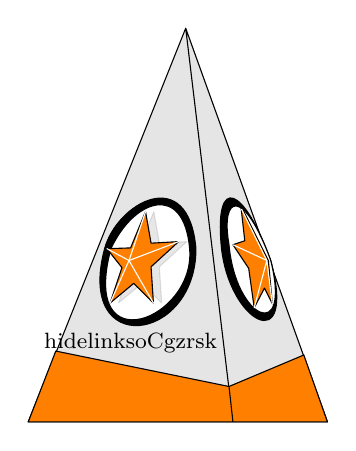
\begin{tikzpicture}[line join = round, line cap=round, >=stealth, font=\footnotesize, scale=1]
		\draw[fill=black!10]
			(-1.30,-1.00)--(0.70,4.00)--(1.30,-1.00)--cycle
			(0.70,4.00)--(2.50,-1.00)--(1.30,-1.00)--cycle;
		\draw[fill=orange]  
			(2.20,-0.15)--(2.50,-1.00)--(1.30,-1.00)--(1.25,-0.55)--cycle
			(1.30,-1.00)--(1.25,-0.55)--(-0.95,-0.10)--(-1.30,-1.00)--cycle;
		\draw[fill=black] 
			(-0.33,1.20)..controls +(75:0.6) and +(95:1.1)..(0.83,1.2)
			..controls +(-90:1.2) and +(-105:1.45)..cycle;
		\draw[fill=white]
			(-0.25,1.20)..controls +(65:0.7) and +(95:0.85)..(0.75,1.2)
			..controls +(-85:0.9) and +(-105:1.53)..(-0.25,1.20);
		\draw[fill=black!91,opacity=0.1,xshift=3pt]
			(-0.30,1.20)--(0.00,1.21)--(0.19,1.67)--(0.26,1.27)--(0.61,1.29)--(0.26,0.97)--(0.29,0.51)--(0.04,0.76)--(-0.26,0.51)--(-0.11,0.96)--cycle;
		\draw[fill=orange] 
			(-0.30,1.20)--(0.00,1.21)--(0.19,1.67)--(0.26,1.27)--(0.61,1.29)--(0.26,0.97)--(0.29,0.51)--(0.04,0.76)--(-0.26,0.51)--(-0.11,0.96)--cycle;
		\draw[white] 
			(-0.02,1.05)--(-0.30,1.20)
			(-0.02,1.05)--(0.19,1.67)
			(-0.02,1.05)--(0.61,1.29)
			(-0.02,1.05)--(0.29,0.51)
			(-0.02,1.05)--(-0.26,0.51);
		\draw[fill=black]
			(1.15,1.25)..controls +(95:0.9) and +(110:1)..(1.78,1.05)
			..controls +(-75:1.3) and +(-85:1).. cycle;
		\draw[fill=white]
			(1.25,1.25)..controls +(100:0.65) and +(110:1)..(1.78,1.05)
			..controls +(-76:1.1) and +(-85:0.95)..cycle;
		\draw[fill=orange]
			(1.75,1.05)--(1.40,1.75)--(1.45,1.30)--(1.30,1.25)--(1.50,0.95)--(1.57,0.45)--(1.70,0.70)--(1.80,0.50)--cycle;
		\draw[white]
			(1.73,1.05)--(1.41,1.7)
			(1.73,1.05)--(1.30,1.25)
			(1.73,1.05)--(1.57,0.45)
			(1.73,1.05)--(1.80,0.50);
		\path (0,0) node{\hypersetup{hidelinks}\href{oCgzrsk}{ }};
	\end{tikzpicture}
\hspace*{1cm}
	\begin{tikzpicture}[line join=round, line cap=round, font=\footnotesize, scale=0.8]
		\path
			(0:0) coordinate (A)
			($(A)+(-55:2.1)$) coordinate (B)
			($(A)+(0:4)$) coordinate (C)
			($(A)!.5!(B)$) coordinate (O1)
			($(B)!.5!(C)$) coordinate (O2)
			(intersection of C--O1 and A--O2) coordinate (O)
			(O)++(90:4.8) coordinate (S)
			(A)--(B)--([turn]-90:0.5cm) coordinate (B1)
			(B)--(A)--([turn]90:0.5cm) coordinate (A1)
			%	(A1)--(B1)node[midway,sloped,below]{$7$ cm}
			%	(O1)--(S)node[midway,sloped,above]{$11$ cm}
		;
		\draw[dashed] (A)--(C)--(O1) (S)--(O);
		\draw 
			(A)--(B)--(C)
			(A)--(S)--(B) (S)--(C) (S)--(O1)
		;
		\draw pic[draw,angle radius=2mm]{right angle=S--O1--A};
		\draw pic[draw,angle radius=2mm]{right angle=C--O--S};
		\foreach \x/\g/\t in {S/90/S,A/180/D,B/-90/E,C/0/F,O1/-120/I,O/-90/O} 
		\draw[fill=black] (\x) circle (.05) +(\g:.3) node{$\t$};		%0.05
	\end{tikzpicture}
\end{center}
	\loigiai{
		Diện tích xung quanh của chóp là $\dfrac{1}{2} \cdot 90 \cdot 60 \cdot 3 = 8\,100$ (cm$^2$).	
	}
\end{bt}

% Bài 4
\begin{bt}%[Dự án EX-8-Đề Cương Toán 8]%[Huu Son]%[8H1V2-3]
	Fansipan là đỉnh núi cao nhất của Việt Nam với độ cao $3\,143$ m, nằm trong dãy núi Hoàng Liên Sơn. Trên đỉnh Fansipan có đặt một cột mốc dạng hình chóp tam giác đều bằng inox (hình bên). Biết cột mốc có mặt đáy là một tam giác đều cạnh $60$ cm, chiều cao của mỗi mặt bên là $1$ m. Tính diện tích xung quanh của cột mốc nêu trên theo đơn vị mét vuông.
\begin{center}
	\begin{tabular}{p{5cm}p{5cm}}
		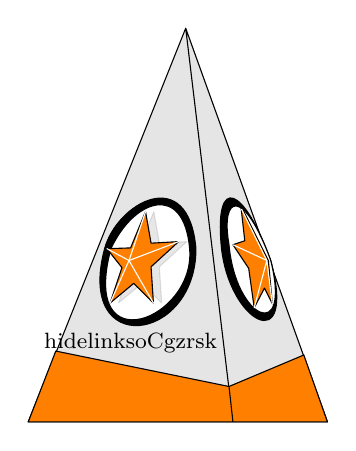
\begin{tikzpicture}[line join = round, line cap=round, >=stealth, font=\footnotesize, scale=1]
			\draw[fill=black!10]
				(-1.30,-1.00)--(0.70,4.00)--(1.30,-1.00)--cycle
				(0.70,4.00)--(2.50,-1.00)--(1.30,-1.00)--cycle;
			\draw[fill=orange]  
				(2.20,-0.15)--(2.50,-1.00)--(1.30,-1.00)--(1.25,-0.55)--cycle
				(1.30,-1.00)--(1.25,-0.55)--(-0.95,-0.10)--(-1.30,-1.00)--cycle;
			\draw[fill=black] 
				(-0.33,1.20)..controls +(75:0.6) and +(95:1.1)..(0.83,1.2)
				..controls +(-90:1.2) and +(-105:1.45)..cycle;
			\draw[fill=white]
				(-0.25,1.20)..controls +(65:0.7) and +(95:0.85)..(0.75,1.2)
				..controls +(-85:0.9) and +(-105:1.53)..(-0.25,1.20);
			\draw[fill=black!91,opacity=0.1,xshift=3pt]
				(-0.30,1.20)--(0.00,1.21)--(0.19,1.67)--(0.26,1.27)--(0.61,1.29)--(0.26,0.97)--(0.29,0.51)--(0.04,0.76)--(-0.26,0.51)--(-0.11,0.96)--cycle;
			\draw[fill=orange] 
				(-0.30,1.20)--(0.00,1.21)--(0.19,1.67)--(0.26,1.27)--(0.61,1.29)--(0.26,0.97)--(0.29,0.51)--(0.04,0.76)--(-0.26,0.51)--(-0.11,0.96)--cycle;
			\draw[white] 
				(-0.02,1.05)--(-0.30,1.20)
				(-0.02,1.05)--(0.19,1.67)
				(-0.02,1.05)--(0.61,1.29)
				(-0.02,1.05)--(0.29,0.51)
				(-0.02,1.05)--(-0.26,0.51);
			\draw[fill=black]
				(1.15,1.25)..controls +(95:0.9) and +(110:1)..(1.78,1.05)
				..controls +(-75:1.3) and +(-85:1).. cycle;
			\draw[fill=white]
				(1.25,1.25)..controls +(100:0.65) and +(110:1)..(1.78,1.05)
				..controls +(-76:1.1) and +(-85:0.95)..cycle;
			\draw[fill=orange]
				(1.75,1.05)--(1.40,1.75)--(1.45,1.30)--(1.30,1.25)--(1.50,0.95)--(1.57,0.45)--(1.70,0.70)--(1.80,0.50)--cycle;
			\draw[white]
				(1.73,1.05)--(1.41,1.7)
				(1.73,1.05)--(1.30,1.25)
				(1.73,1.05)--(1.57,0.45)
				(1.73,1.05)--(1.80,0.50);
			\path (0,0) node{\hypersetup{hidelinks}\href{oCgzrsk}{ }};
		\end{tikzpicture}
	&
	\begin{tikzpicture}[line join=round, line cap=round, font=\footnotesize, scale=0.8]
		\path
			(0:0) coordinate (A)
			($(A)+(-35:3.1)$) coordinate (B)
			($(A)+(0:4)$) coordinate (C)
			($(A)!.5!(B)$) coordinate (O1)
			($(B)!.5!(C)$) coordinate (O2)
			(intersection of C--O1 and A--O2) coordinate (O)
			(O)++(90:4.8) coordinate (S)
			(A)--(B)--([turn]-90:0.5cm) coordinate (B1)
			(B)--(A)--([turn]90:0.5cm) coordinate (A1)
			(S)--(O1)node[midway,sloped,above]{$1$ m}
			(B)--(C)node[midway,sloped,below]{$60$ cm}
		;
		\draw[dashed] (A)--(C)--(O1) (S)--(O);
		\draw 
			(A)--(B)--(C)
			(A)--(S)--(B) (S)--(C) (S)--(O1)
		;
		\draw pic[draw,angle radius=2mm]{right angle=S--O1--A};
		\draw pic[draw,angle radius=2mm]{right angle=C--O--S};
		\foreach \x/\g/\t in {S/90/S,A/180/D,B/-90/C,C/0/B,O1/-120/H} 
		\draw[fill=black] (\x) circle (.05) +(\g:.3) node{$\t$};		%0.05
	\end{tikzpicture}
	\end{tabular}
	\end{center}
	\loigiai{
		Diện tích xung quanh của cột mốc là \\
		\hspace*{0.4cm}	$\left(\dfrac{1}{2} \cdot 0{,}6 \cdot 1 \right) \cdot 3 = 0{,}9$ (m$^2$).
	}
\end{bt}

% Bài 5
\begin{bt}%[Dự án EX-8-Đề Cương Toán 8]%[Huu Son]%[8H1V2-3]
\immini[thm]{
	Một chiếc đèn thả trần có dạng hình chóp tam giác đều (hình bên) có độ dài cạnh đáy bằng $20$ cm, chiều cao của đèn bằng $\dfrac{20\sqrt{6}}{3}$ cm. Tính thể tích của chiếc đèn (làm tròn kết đến chữ số hàng đơn vị).
}
{
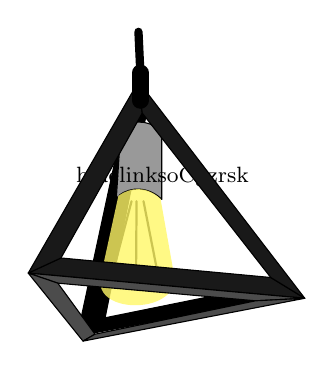
\begin{tikzpicture}[scale=0.8, font=\footnotesize, line join=round, line cap=round, >=stealth]
	%Sau
	\draw[fill=black] (-1.32,-2.38)--(-0.58,1.05)--(-0.22,1.17)--(-0.91,-2.24)--(1.41,-1.77)--(1.98,-1.89)--(-1.19,-2.5)--cycle;
	%Đui đèn
	\draw[fill=black!40] (-0.68,-0.29)..controls (-0.51,-0.16) and (-0.22,-0.15)..(-0.01,-0.36)--(-0.01,0.69)..controls (-0.14,0.88) and (-0.44,0.94)..(-0.66,0.76)--(-0.73,-0.32);
	\path (0,0) node{\hypersetup{hidelinks}\href{oCgzrsk}{ }};
	%Dây tóc
	\draw[thick] (-0.49,-0.39)--(-0.8,-1.57);
	\draw[thick] (-0.41,-0.39)--(-0.42,-1.73);
	\draw[thick] (-0.3,-0.39)--(-0.06,-1.61);
	\draw plot[smooth, tension=.7] coordinates {(-0.8,-1.57) (-0.67,-1.7) (-0.42,-1.73) (-0.21,-1.72) (-0.06,-1.61)};
	%Bóng đèn
	\fill[white!40!yellow,opacity=0.8]
		(-0.68,-0.29)..controls (-0.51,-0.18) and (-0.27,-0.13)..(-0.03,-0.35)
		-- (0.18,-1.53)..controls (0.33,-2.18) and (-1.11,-2.22)..(-0.98,-1.59)--(-0.7,-0.31);
	%Mặt trước
	\draw[fill=black!90] (-2.13,-1.53)--(-1.61,-1.29)--(1.72,-1.6)--(2.26,-1.93)--cycle;
	\draw[fill=black!90] (-2.13,-1.53)--(-1.61,-1.29)--(-0.32,1.01)--(-0.38,1.51)--cycle;
	\draw[fill=black!90] (-0.38,1.51)--(-0.32,1.01)--(1.72,-1.6)--(2.26,-1.93)--cycle;
	%Đáy
	\draw[fill=black!70] (-2.13,-1.53)--(-1.66,-1.69)--(1.48,-1.97)--(2.26,-1.93)--cycle;
	\draw[fill=black!70] (-2.13,-1.53)--(-1.66,-1.69)--(-1.07,-2.5)--(-1.26,-2.61)--cycle;
	\draw [fill=black!70] (-1.26,-2.61)--(-1.07,-2.5)--(1.48,-1.97)--(2.26,-1.93)--cycle;
	%Dây điện
	\draw[line width=6pt] (-0.35,1.21)--(-0.35,1.65);
	\draw[line width=3pt](-0.35,1.65)--(-0.38,2.3);
\end{tikzpicture}
}
	\loigiai{
	Thể tích của chiếc đèn là \\
	\hspace*{0.4cm} $V=\dfrac{1}{3} \cdot \dfrac{20\sqrt{3}}{4} \cdot \dfrac{20\sqrt{6}}{3} \approx 47$ (cm$^3$).
}
\end{bt}

% Bài 6
\begin{bt}%[Dự án EX-8-Đề Cương Toán 8]%[Huu Son]%[8H1V2-3]
\immini[thm]{
	Bạn Trang cắt miếng bìa hình tam giác đều cạnh dài $20$ cm và gấp lại theo các dòng kẻ nét đứt như hình vẽ để được hình chóp tam giác đều. Tính diện tích xung quanh của hình chóp tam giác đều tạo thành. Cho biết $\sqrt{75}\approx 8{,}66$.
}
{
\begin{tikzpicture}[line join=round, line cap=round, font=\footnotesize, scale=1]
\path 
	(0,0) coordinate (A)
	(-60:4) coordinate (C)
	(-120:4) coordinate (B)
;
\draw (A)--(B)--(C)--cycle;
\draw[dashed] ($(A)!0.5!(B)$)--($(A)!0.5!(C)$)--($(B)!0.5!(C)$)--cycle;
\end{tikzpicture}
}
	\loigiai{
		Độ dài cạnh của hình chóp là $10$ cm. \\
		Độ dài trung đoạn $\sqrt{10^2-5^2} = \sqrt{75} \approx 8{,}66$ (cm). \\
		Diện tích một mặt bên của hình chóp tam giác đều là \\
		\hspace*{0.4cm} $\dfrac{1}{2} \cdot 10 \cdot 8{,}66 = 43{,}3$ (cm$^2$). \\
		Diện tích xung quanh của hình chóp tam giác đều là \\
		\hspace*{0.4cm} $43{,}3 \cdot 3 = 129{,}9$ (cm$^2$).
	}
\end{bt}

% Bài 7
\begin{bt}%[Dự án EX-8-Đề Cương Toán 8]%[Huu Son]%[8H1V2-3]
	Kim tự tháp Kheops – Ai Cập có dạng hình chóp tứ giác đều có chiều cao bằng $139$ m và cạnh đáy bằng $230$ m. Tính thể tích của kim tự tháp này (kết quả làm tròn đến hàng nghìn, với đơn vị là m$^3$).
\begin{center}
	\begin{tikzpicture}[line join=round, line cap=round, font=\footnotesize, scale=0.5]
		\def\canhAB{4};\def\canhBC{10};\def\gocABC{30};\def\h{7};
		\coordinate (B) at (0,0);
		\coordinate (A) at ($(B)+(\gocABC:\canhAB)$);
		\coordinate (C) at ($(B)+(0:\canhBC)$);
		\coordinate (D) at ($(A)+(0:\canhBC)$);
		\coordinate (O) at ($(A)!0.5!(C)$);
		\coordinate (S) at ($(O)+(90:\h)$);
		\draw [pattern=bricks](S)--(B)--(C)--cycle;
		\draw [pattern=bricks, pattern color=gray] (S)--(D)--(C)--cycle;
%		\foreach \i/\g in {A/120, B/0, C/60, D/-60, O/-90, S/45}
%			\draw[fill=white](\i) circle (1.5pt) ($(\i)+(\g:4.0mm)$) node[scale=1]{$\i$}; %3.5
	\end{tikzpicture}
	\hspace*{1cm}
	\begin{tikzpicture}[line join=round, line cap=round, font=\footnotesize, scale=0.5]
		\def\canhAB{4};\def\canhBC{10};\def\h{7};\def\gocABC{30};
		\coordinate (B) at (0,0);
		\coordinate (A) at ($(B)+(\gocABC:\canhAB)$);
		\coordinate (C) at ($(B)+(0:\canhBC)$);
		\coordinate (D) at ($(A)+(0:\canhBC)$);
		\coordinate (O) at ($(A)!0.5!(C)$);
		\coordinate (S) at ($(O)+(90:\h)$);
		\draw (S)--(B)--(C)--(D)--(S)--(C);
		\draw[dashed] (B)--(A)--(D) (S)--(A)--(C) (B)--(D) (S)--(O);
		\foreach \x/\y in {A/140,B/-90,C/-90,D/0,S/90,O/-90}{
			\fill (\x) circle (0.05) ($(\x)+(\y:0.4cm)$) node{$\x$};}
		\path ($(S)!0.3!(O)$)--(O)node[sloped, above, midway]{$139$ cm};
		\path (B)--(C)node[below, midway]{$230$\,cm};
		\foreach \x/\y/\z in {S/O/D}
			\path pic[draw,angle radius=5pt]{right angle= \x--\y--\z};
	\end{tikzpicture}
\end{center}
	\loigiai{
		Thể tích của kim tự tháp là \\
		\hspace*{0.4cm} $V=\dfrac{1}{3}\cdot230^2\cdot139\approx 2\,451\,000$ (m$^3$).
	}
\end{bt}

% Bài 8
\begin{bt}%[Dự án EX-8-Đề Cương Toán 8]%[Huu Son]%[8H1V2-3]
	Một cửa hàng bán lều ngủ cho trẻ em có dạng hình chóp tứ giác đều có cạnh đáy dài $1{,}6$\,m và các mặt bên là những tam giác cân có chiều cao $1{,}4$\,m. Tính diện tích vải xung quanh lều.
	\begin{center}
		\begin{tikzpicture}[line join=round, line cap=round, >=stealth, font=\footnotesize, scale=.8]
			\path 
				(0,0) coordinate (A)
				(10:5) coordinate (B)
				(-30:3) coordinate (D)
				($(B)+(D)-(A)$) coordinate (C)
				(60:6) coordinate (S)
				($(C)!.5!(D)$) coordinate (M)
			;
			\foreach \i in {A,C,D,M}
				\draw[thick] (S)--(\i);
			\draw[thick] (A)--(D)node[left,pos=.6,xshift=-5]{$1{,}6$\,m}--(C);
			\path (S)--(M)node[left,pos=.6,xshift=-2]{$1{,}4$\,m};
			\draw[thin, dashed] (S)--(B) (A)--(B)--(C);			
			\draw pic[thick, draw, angle radius=5pt]{right angle=S--M--C};			
			\foreach \x in {A,B,C,D,S,M} 
				\fill (\x) circle (0.05);
		\end{tikzpicture}
	\end{center}
	\loigiai{
		Diện tích vải xung quanh của lều là \\
		\hspace*{0.4cm} $\left(\dfrac{1}{2} \cdot 1{,}6 \cdot 1{,}4\right) \cdot 4 = 4{,}48$ (m$^2$).
	}
\end{bt}

% Bài 9
\begin{bt}%[Dự án EX-8-Đề Cương Toán 8]%[Huu Son]%[8H1H2-3]
\immini[thm]{
	Một cái lều ở trại hè của học sinh có dạng hình chóp tứ giác đều kèm theo các kích thước như hình vẽ. Tính diện tích vải bạt cần thiết để dựng lều (không tính đến đường viền, nếp gấp), biết chiều cao của mặt bên xuất phát từ đỉnh của chiếc lều là $2{,}24$\,m và lều này không có đáy.
}
{
\begin{tikzpicture}[line join=round, line cap=round, font=\footnotesize, scale=0.75]
	\path
		(0,0) coordinate (A)
		(3,-3) coordinate (B)
		(7,0) coordinate (D)
		($(B)+(D)-(A)$) coordinate (C)
		($(A)!0.5!(C)$) coordinate (O)
		($(O)+(0,5)$) coordinate (S)
		($(A)!1/3!(B)$) coordinate (x)
		($(A)!2/3!(B)$) coordinate (y)
		(x)+(40:2) coordinate (z)
		($(y)!1/2!(z)$)++(-40:1.1) coordinate (t)
	;
	\draw(S)--(A) (S)--(B) (S)--(C) (A)--(x)--(z)--(y)--(B) (B)--(C)node[below,midway]{$2$\,m} (S)--($(B)!0.5!(C)$)node[shift=(70:1cm),rotate=-75]{$2{,}24$\,m};
	\draw[dashed,thin] (A)--(D) (C)--(D) (S)--(D)  (B)--(D) (S)--(O);
	\draw (z) to[out=-85,in=140] (t) to[out=-180,in=40] (y);
		\draw pic[draw,angle radius=0.5cm]{right angle=D--C--B};
	\foreach \j in {A,B,C,D}{\path (S)--(\j)node[midway,sloped,scale=0.7]{$|$};}
	\foreach \i in {A,B,C}
		\draw[line width=2pt] ($(\i)+(-80:0.3)$)--($(\i)+(100:0.3)$);
%	\foreach \i/\g in {A/120, B/0, C/60, D/-60, O/-90, S/45}
%		\draw[fill=white](\i) circle (1.5pt) ($(\i)+(\g:4.0mm)$) node[scale=1]{$\i$}; %3.5
\end{tikzpicture}
}
	\loigiai{
	Vì cái lều ở trại hè của học sinh có dạng hình chóp tứ giác đều nên các mặt bên là các tam giác cân bằng nhau. \\
	Diện tích vải bạt cần thiết để dựng lều là \\
	\hspace*{0.4cm} $\left(\dfrac{1}{2} \cdot 2 \cdot 2{,}24\right) \cdot 4=8{,}96$ (m$^2$).
	}
\end{bt}

% Bài 10
\begin{bt}%[Dự án EX-8-Đề Cương Toán 8]%[Huu Son]%[8H1C1-3]
\immini[thm]{
	Bác An làm một chiếc hộp gỗ có dạng hình chóp tứ giác đều như hình vẽ. Bác An muốn sơn tất cả các mặt của hộp gỗ. Cứ mỗi mét vuông sơn cần trả $30\,000$ đồng (tiền sơn và tiền công). Hỏi bác An cần phải trả chi phí là bao nhiêu, biết $PQ = 5$ m và $SH = 3$ m.
}
{
\begin{tikzpicture}[>=stealth,line join=round,line cap=round,font=\footnotesize,scale=1]
	\tikzset{
		pics/hinhChopTuGiacDeu/.style  n args={6}{
			code={
				\tikzset{
					declare function={a=2.5;b=2.5;h=3;goc=-140;}
				}	
				\path 
				(0,0)coordinate (#1)+(-35:b)coordinate (#2)+(goc:a)coordinate (#4)			
				($(#2)+(#4)-(#1)$)coordinate (#3)
				(intersection of #1--#3 and #2--#4)coordinate (#5) ($(#5)+(90:h)$)coordinate (#6)
				;
			}
	}}
	\path 
	(0,0)pic {hinhChopTuGiacDeu={N}{P}{Q}{M}{O}{S}}
	($(M)!.5!(Q)$)coordinate (H)	
	;	
	\fill[left color=brown!80!black,middle color=brown!85!black,right color=brown!60!white] (S)--(M)--(Q) ;
	\draw[brown!80!black] pic[draw,angle radius=2mm,angle eccentricity=2.4]{right angle=S--H--Q};
	\fill[left color=brown!70!black,middle color=brown!85!black,right color=brown] (S)--(Q)--(P);
	\foreach \pointo/\pointt in {S/P,S/Q,S/M,M/Q,Q/P,S/H}{
		\draw[fill=black,brown!80!black,thick](\pointo)--(\pointt);
	}
	\foreach \pointo/\pointt in {S/N,N/M,N/P}{
		\draw[fill=black,dashed,brown!80!black,thick](\pointo)--(\pointt);
	}
\end{tikzpicture}
\begin{tikzpicture}[>=stealth,line join=round,line cap=round,font=\footnotesize,scale=1]
	\tikzset{
		pics/hinhChopTuGiacDeu/.style  n args={6}{
			code={
				\tikzset{
					declare function={a=2.5;b=2.5;h=3;goc=-140;}
				}	
				\path 
				(0,0)coordinate (#1)+(-35:b)coordinate (#2)+(goc:a)coordinate (#4)			
				($(#2)+(#4)-(#1)$)coordinate (#3)
				(intersection of #1--#3 and #2--#4)coordinate (#5) ($(#5)+(90:h)$)coordinate (#6)
				;
			}
	}}
	\path 
	(0,0)pic {hinhChopTuGiacDeu={N}{P}{Q}{M}{O}{S}}
	($(M)!.5!(Q)$)coordinate (H)
	pic[draw,angle radius=2mm,angle eccentricity=2.4]{right angle=S--H--Q}
	;	
	\path (S)--(H)node[pos=.7,above,sloped]{$3$ m} (Q)--(P)node[pos=.5,below,sloped]{$5$ m};
	\foreach \pointo/\pointt in {S/P,S/Q,S/M,M/Q,Q/P,S/H}{
		\draw[fill=black](\pointo)--(\pointt);
	}
	\foreach \pointo/\pointt in {S/N,N/M,N/P}{
		\draw[fill=black,dashed](\pointo)--(\pointt);
	}
	\foreach \point/\goc in {S/90,N/135,M/190,P/-20,Q/-90,H/190}{
		\draw[fill=black](\point)circle(.8pt)+(\goc:2mm)node[scale=.8]{$\point$};
	}
\end{tikzpicture}	
}
	\loigiai{
	Ta có $S_{\text{tp}}=S_{\text{xq}}+S_{\text{đáy}}=4 \cdot \dfrac{1}{2} \cdot 3 \cdot 5+5^2=55$ (m$^2$). \\
	Vậy Bác An cần phải trả chi phí là $55\cdot 30\,000=1\,650\,000$ (đồng).
	}
\end{bt}






% In đáp án trắc nghiệm
\Closesolutionfile{ans}
\indapan{6}{ans/ans-8C2-OTC}